\documentclass[main.tex]{subfiles}
\begin{document}


\chapter{Concept} \label{chap:Concept}


\begin{figure}[!ht]
    \centering
    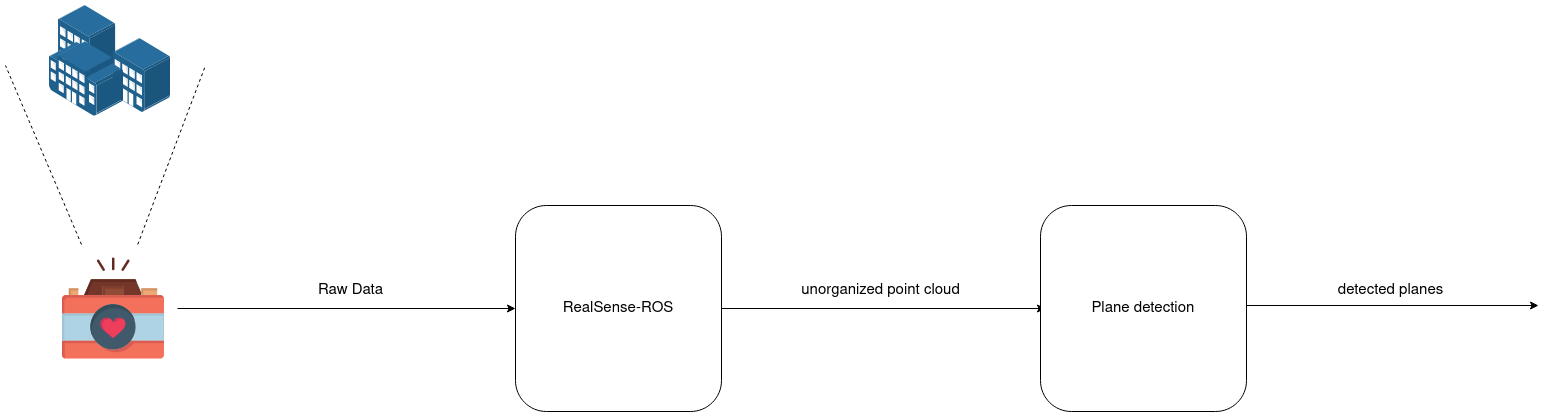
\includegraphics[width=15 cm]{images/concept.png}
    \caption{A camera records an environment. The recorded data is either preprocessed, or passed directly to the plane detection algorithm.
        The resulting planes are subsequently exported to an arbitrary application.}
    \label{fig:concept}
\end{figure}


% \section{Scenario / UseCase}

Within a given use case or scenario, the user records the surroundings with a camera, and the raw data is either
directly, or after some preprocessing steps, passed to a plane detection algorithm, which then hands the detected planes to an application for further use.
This application could use those planes to define the playable area in an augmented reality (AR) video game or alternatively build a digital floor
plan, or 3-D model, of an apartment.

Especially in scenarios where the user moves through the environment, the time between recording and the planes reaching the application is crucial.
If an autonomous car drives through an urban environment, the delay must be as short as possible to avoid a collision with a wall the car has not yet detected.

The problem can therefore be defined in such a way that planes must be detected in real-time and at the same time be sufficiently precise for the given use case.

% To optimize the entire process, shown in Figure~\ref{fig:concept}, this work will aim to answer the question of to what extent precise real-time plane detection is feasible. 
% NOTE alternative: 
To optimize the entire process, shown in \ref{fig:concept}, this work will focus on the plane detection step (green).

Furthermore, we focus on indoor environments, as motivated by Chapter~\ref{chap:Introduction}.
This includes the buildings we encounter in our normal lives, whether it is the home we live in, the office we work in, or a stripped-down version of a building during construction.




\subsection{Used Sensors}
% FIXME how do I reference step one
To efficiently tackle the previously defined problem, and according to figure~\ref{fig:concept}, \textcolor{red}{phase 1}, we need a camera sensor to record the environment and obtain data to detect planes therein.

Numerous cameras suffice for this task, each of which varies in different aspects.
For this work, we use the Intel RealSense T256 Tracking Camera and the Intel RealSense D455 RGB-D Camera, because of their compatibility,
since the T256 can be used in combination with any depth camera from the D400 series.

Since we are especially interested in the detection of planes in complete environments, it is necessary to be able to build a map out of the data the cameras
record continuously.
In addition to the cameras, the Intel RealSense software provides a way to perform map assembly, \textcolor{red}{siehe concept figure, step 2}.
%  neuen absatz mit this is why anfangen ist meh
We integrate \textit{realsense-ros}, the ROS wrapper of Intel RealSense, into our process of plane detection.

Realsense-ros internally uses a SLAM(Simultaneous Mapping and Localization) algorithm called RTAB-MAP \cite{Labbé_Michaud_2019} for map-building.
RTAB-MAP is responsible for building a coherent map from a continuous stream of data that is being recorded and published by the two cameras.
It is worth noting, that the success of this work does not depend on the specific SLAM algorithm being chosen. We select RTAB-MAP because
it is already included in the RealSense package and its reported performance suffices for this work, primarily since we don't focus on SLAM
algorithms in this work.

Mit intel realsense und rtabmap lässt sich Figure~\ref{fig:concept} konkreter beschreiben, siehe Figure~\ref{fig:concept_spec}

\begin{figure}[!ht]
    \centering
    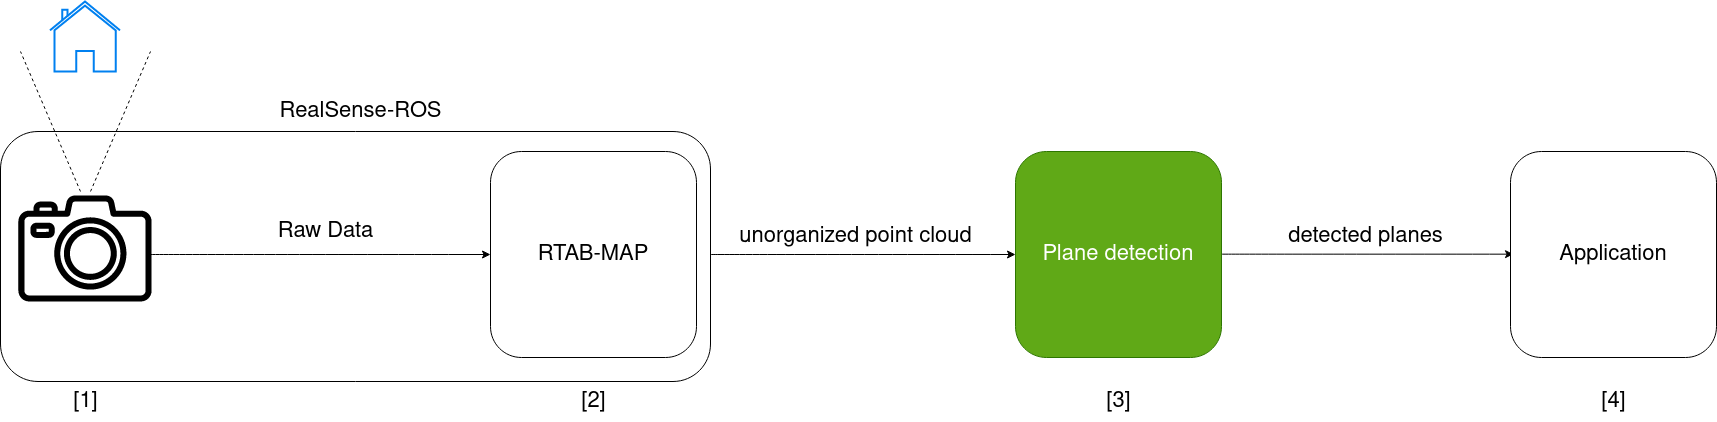
\includegraphics[width=15 cm]{images/concept_specific.png}
    \caption{Updated process with sensors and what not}
    \label{fig:concept_spec}
\end{figure}

\section{Selection Plane Detection Algorithms}
Naturally, appropriate algorithms are needed to perform real-time plane detection, as depicted in Figure~\ref{fig:concept}, \textcolor{red}{step 3}.
First, we define meaningful criteria to select plane detection algorithms. Then, we use these criteria to select appropriate algorithms from the list of algorithms.

\subsection*{Type of Input}
Usually, the data representation of the recorded environment passed to the plane detection algorithm falls under one of three categories:
\begin{itemize}
    \item \textit{unorganized} or \textit{unstructured point cloud} (UPC)
    \item \textit{organized} or \textit{structured point cloud} (OPC)
    \item \textit{(depth-) image} (D-/I)
\end{itemize}

As stated before, we focus on detecting planar structures in the entire environment rather than just distinct segments thereof.
In addition, only the unorganized/unstructured point clouds offer a complete view of the recorded environment.
% NOTE kommt später: Therefore, we disregard all algorithms which do not expect an unorganized point cloud as input.


\subsection*{Detected Plane Format}
Which specific representation the detected planes take the form of is also essential.
If no uniform output type can be determined, consequently, no uniform metric for comparison can also be found.
Since the algorithms process point clouds, we choose to stay within the realm of points, i.e., an arbitrary plane should be
represented by the set of points included in the plane (inliers).
The representation, being a list of points, enables further processing of the detected planes.
A list of points would, in contrast to some plane equation, enable us to detect holes in planes, e.g.,
an open door or window, which can be helpful in any use case involving remodeling architectural elements.
It also allows further filtering of planes based on a density value that we can calculate over the bounding
box and the number of points, e.g., removing planes with a density lower than a certain threshold.


\subsection*{Learning based}\label{subsec_learning_based}
Learning-based methods, e.g. Deep learning, generally have varying levels of bias, depending on the training data. 
Another reason against the use of learning-based methods is that we choose not to require a GPU to replicate our findings.
% FIXME  kann ich das so sagen? -> we choose not to require a GPU to replicate our findings.

\subsection*{Availability}
Lastly, we include the availability of an algorithm in our set of criteria.
Each algorithm to be compared needs to run on the same system to exclude the underlying hardware as a factor from any experiments.\\

\section{Algorithms?}
\subsection*{RSPD - Robust Statistics Approach for Plane Detection}

\subsection*{OPS - Oriented Point Sampling}

\subsection*{3DKHT - 3-D Kernel-based Hough Transform}
With 3D-KHT, as with other octree-based methods, the performance depends, to some degree, on the level of subdivision.
In the provided implementation, the octree keeps dividing until either the number of points in the current node is lower than a set minimum, or the
level of an octree node is higher than a predefined maximum.

% FIXME wahrscheinlich muss ich sagen woran ich das getestet habe oder?
A total of six different presets of parameters are included with the official implementation.
Since this work does not focus on the evaluation and analysis of a single method, we performed experiments with all presets on a data set, the
results thereof can be seen in Figure ~\ref{fig:3dkht_params}
\begin{figure}[!h]
    \centering
    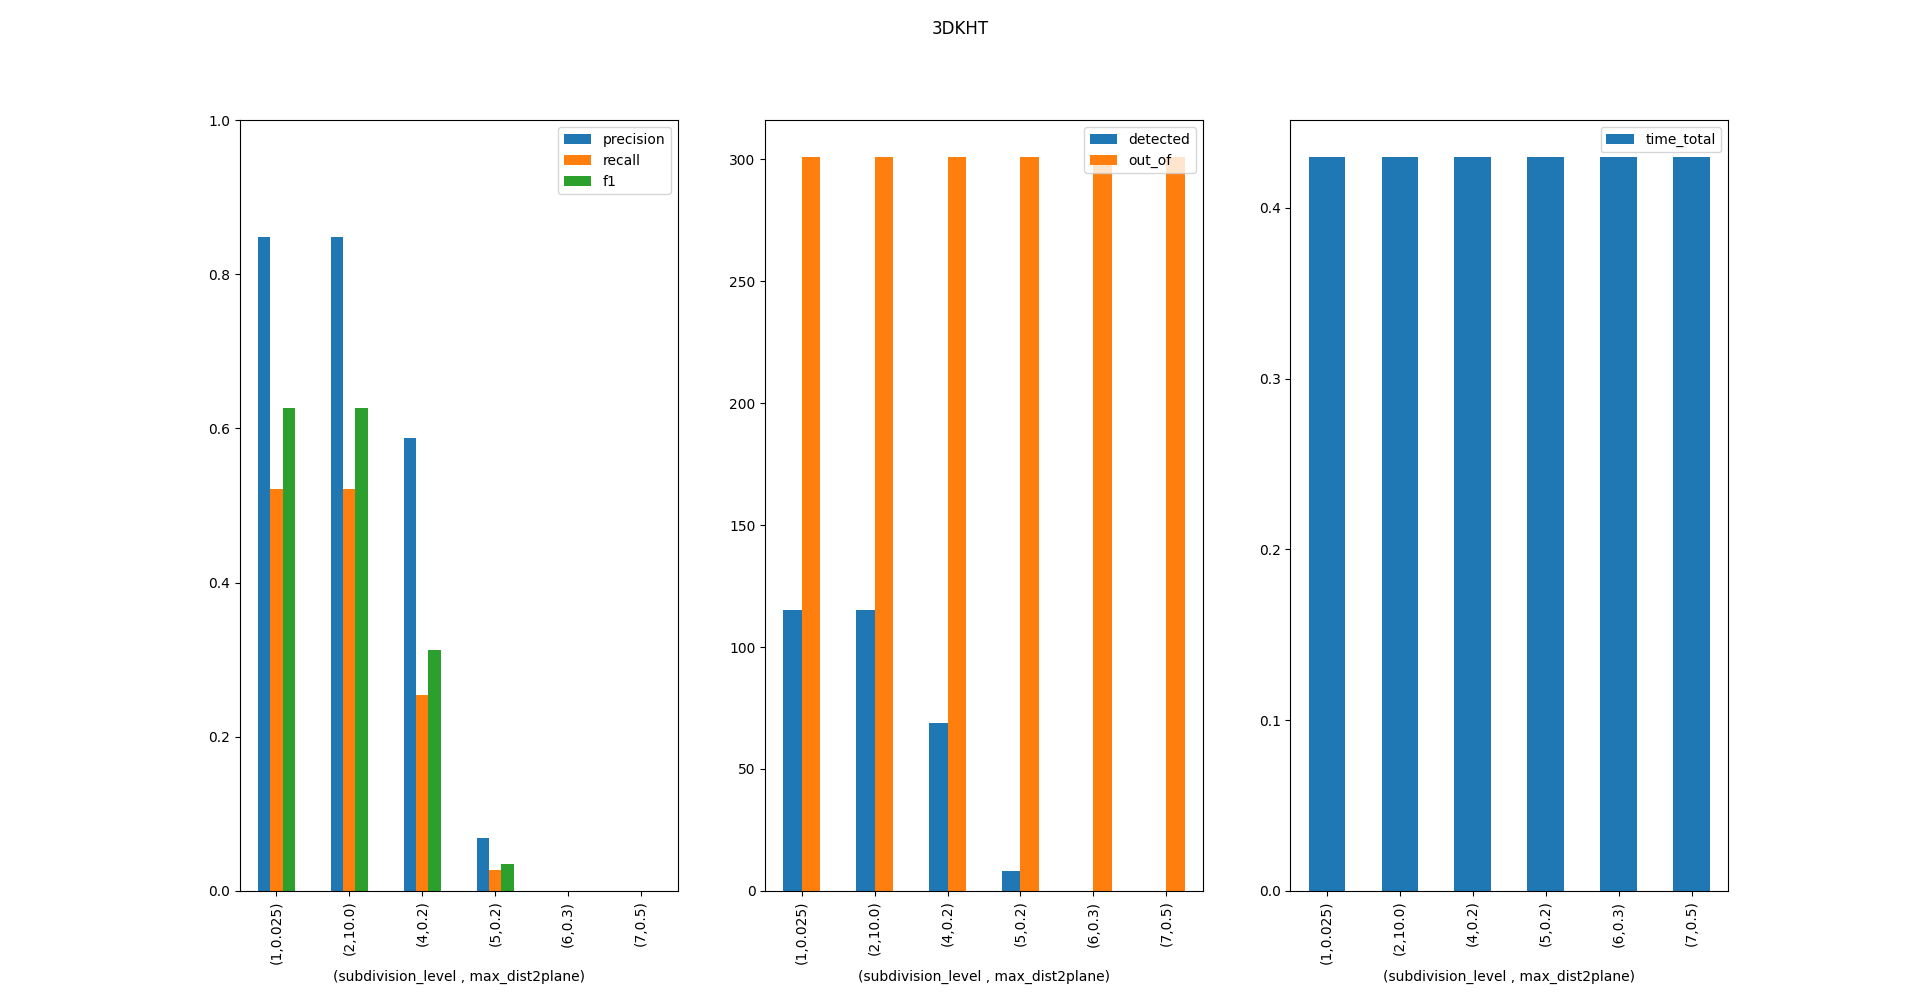
\includegraphics[width=15 cm]{params_3dkht.png}
    \caption{Results of 3D-KHT for different pre-set subdivision values}
    \label{fig:3dkht_params}
\end{figure}

% FIXME speculation?
Because the leftmost two presets, with an octree subdivision value of 1 and 2, respectively, seem to yield similar results, but a higher value of subdivision
might result in better performance in larger point clouds, we will perform all calculations of 3D-KHT with an octree subdivision value of 2.

\subsection*{OBRG - Octree-based Region Growing}
\subsection*{PEAC - Probabilistic Agglomerative Hierarchical Clustering}

\subsection{Summary: Plane Detection Algorithms}

\begin{table}[!ht]
    \centering
    \begin{tabular}{|c|c|c|c|c|c}
        \hline
                                                                         & \textbf{Input Data} & \textbf{Plane format}                 & \textbf{Learning-Based} & \textbf{Availability} \\ \hline
        \textbf{RSPD} \cite{Araújo_Oliveira_2020}                        & UPC                 & inliers                               & N                       & Y                     \\ \hline
        \textbf{OPS} \cite{Sun_Mordohai_2019}                            & UPC                 & inliers                               & N                       & Y                     \\ \hline
        \textbf{3DKHT} \cite{Limberger_Oliveira_2015}                    & UPC                 & inliers                               & N                       & Y                     \\ \hline
        \textbf{OBRG} \cite{Vo_Truong-Hong_Laefer_Bertolotto_2015}       & UPC                 & inliers                        & N                       & N                     \\ \hline
        \textbf{PEAC} \cite{Feng_Taguchi_Kamat_2014}                     & OPC                 & inliers                               & N                       & Y                     \\ \hline
        \textbf{CAPE} \cite{Proença_Gao_2018}                            & OPC                 & normal, d                             & N                       & Y                     \\ \hline
        \textbf{SCH-RG} \cite{Mols_Li_Hanebeck_2020}                     & OPC                 & inliers?                              & N                       & N                     \\ \hline
        \textbf{D-KHT}  \cite{Vera_Lucio_Fernandes_Velho_2018}           & DI                  & inliers                               & N                       & Y                     \\ \hline
        \textbf{DDFF} \cite{Roychoudhury_Missura_Bennewitz_2021}         & DI                  & \textcolor{red}{indices}              & N                       & Y                     \\ \hline
        \textbf{PlaneNet} \cite{Liu_Yang_Ceylan_Yumer_Furukawa_2018}     & I                   & normal, d & Y                       & Y                     \\ \hline
        \textbf{PLaneRecNet} \cite{Xie_Shu_Rambach_Pagani_Stricker_2022} & I                   & ? / -                                 & Y                       & Y                     \\ \hline
        \textbf{PlaneRCNN} \cite{Liu_Kim_Gu_Furukawa_Kautz_2019}         & I                   & normal + ?                            & N                       & Y                     \\ \hline
    \end{tabular}
    \caption{Plane Detection Algorithms}
    \label{tab:my-table}
\end{table}

\subsection*{Summary Plane Detection Algorithms}
To effectively compare the presented algorithms, the data on which each algorithm performs the plane detection should ideally be the same.
Considering algorithms that run on anything other than UPC, would necessitate finding a data set that includes equivalent point clouds for both the structured and the unstructured case.
Since these algorithms would disregard the global structure of the point cloud, we deem them not feasible for our use case and thus exclude them from our evaluation.

% FIXME seems repeating to me, having a paragraph per criteria to reference them here in one single sentence
We exclude learning-based methods for the reasons previously stated in Subsection~\ref{subsec_learning_based}.

For an even comparison, the detected planes would have to be in the same format because, even for the same plane, representations could very well lead to different results, e.g., a plane in cartesian form compared to the same plane, described by its inliers.
Asserting comparability, we exclude all methods which do not offer a plane representation by inliers.

Lastly, writing our own implementation of methods for which no implementation is available or for which the respective publication does not focus on the implementation details would go beyond the scope of this work.
Finally, we end up with, and thus include, the following plane detection algorithms in our evaluation:

\begin{itemize}
    \item RSPD
    \item OPS
    \item 3D-KHT
    \item OBRG
\end{itemize}


\section{Real-Time}
To determine whether or not an algorithm runs in real-time, we must first define the meaning of real-time.

We have to consider possible hardware limitations, data flow, and simply
how often it is needed to perform calculations in correspondence with the given use case.

%TODO Gar nicht mehr unbedingt nötig, wenn die obere grenze eh der SLAM ist, oder? 
%  The D455 has a depth frame rate of up to 90, while the T256 only achieves a maximum frame rate of 30
The recorded raw data is not directly sent to the plane detection algorithm but instead given to RTAB-MAP, which then performs
calculations to update and publish the map.
Therefore, the upper limit is the frequency of how often RTAB-MAP publishes those updates, which by default is once per second.
According to this upper limit, we consider an algorithm \textit{real-time applicable}, if it achieves an average frame
rate of minimum 1, e.g., the algorithm manages to process the entire point cloud and detect all planes within one second.

%TODO  Eig nur needed wenn die algos langsamer sind als 1s ODER sollte die cloud extrem wachsen kann man sich auf die 6 meter beschränken, erstmal aber nicht}\\
% \subsection*{reduktion (opt)}
% We can reduce complexity further by taking the specifications (background)
% of the D455 into account. The RMS error of the D455 is reported to be 2\% at 4 meters distance to the sensor.
% Furthermore, the ideal distance is stated to range between $0.6 - 6$ meters.
% To maintain a dense and precise representation of our environment, we therefore limit the detection of planes to a
% radius of 6 meters from the current position.

\section{Summary}
Many applications have constraints in the form of a temporal component. Applications that include plane detection
are no exception. The calculation of planes is an obvious bottleneck in the procedure shown in Figure~\ref{fig:concept}.
To evaluate to what extent it is possible to perform precise plane detection with a real-time constraint,
we compare selected algorithms.

\end{document}